% ==============================================================
% File     : chapters/07-Architecture.tex
% Date     : 03 Apr. 2022
% Revision : 30 July 2022
% Creator  : Marco Peressutti
% ==============================================================


\chapter{Agent Architecture}
\minitoc

\section{Abtract Architectures}
Let us make formal the abstract view of agents presented so far. First, let us assume that the evironment may be in any of a finite set $E$ if discrete instantaneous states:
\[E = \{e, e',...\}\]
This is a fairly standard modelling assumption, which we can justify by pointing out that any continuous environment can be modelled by a discrete environment to any desired degree of accuracy.

Agents are assumed to have a repertoire of possible actions available to them, which tranform the state of the environment. \\
Let
\[Ac = \{\alpha, \alpha',...\}\]
be the finite set of actions.

The basic model of agents interacting with their environments goes as follow:
\begin{enumerate}
\item The environment starts in some state
\item The agent begins by choosing an action to perform on that state
\item As a result of this action, the environment can respond with a number of possible states, however, only one state will actually result, though, of course, the agent does not know in advance which will it be.
\item On the basis of this second state, the agent again chooses an action to perform.
\item The environment responds with one of a set of possible states
\item ...
\end{enumerate}

A \side{run} ($r$) of an agent in an environment is thus a sequence of interleaved environment states and actions
\[r: e_0 \rightarrow \alpha_0\,e_1\rightarrow \alpha_1\,e_2\rightarrow \alpha_2\,e_3\rightarrow ... \rightarrow \alpha_{u-1}\,e_u\]
Let 
\begin{itemize}
\item $\mathcal{R}$ be the set of all such possible finite sequeces (over $E$ and $Ac$)
\item $\mathcal{R}^{Ac}$ be the subset of these that end with an action
\item $\mathcal{R}^{E}$ be the subset of these that end with an environment state 
\end{itemize}
We will use $r, r', ...$ to stand for members of $\mathcal{R}$.

In order to represent the effect that an agent's actions have on an environment we introduce a \side{state tranformer function}
\[\tau : \mathcal{R}^{Ac}\rightarrow 2^E\]
Thus a state tranformer function maps a run (assumed to end with the action of an agent) to a set of possible environment states, those that could result from performing the action.

There are two important points to note about this definitions:
\begin{itemize}
\item Environments are assumed to be \side{history dependent}, i.e. the next state of an environment is not solely determined by the action performed by the agent and the current state of the environment. The actions made earlier by the agent also play a part in determining the current state
\item This definition allows for \side{non-determinism} in the environment. There is thus uncertainty about the result of performing an action in some state
\end{itemize}

If $\tau(r) 0 \cancel{0}$ where r is assumed to end with an action, then there are no possible successor states to $r$. In this case, we say that the system has ended its run. We will also assume that all runs eventually terminate.

Formally, we say that an environment $Env$ is triple 
\[Env=\langle E, e_0,\tau\rangle\]
where:
\begin{itemize}
\item $E$ is a set of environment states
\item $e_0 \in E$ is an initial state
\item $\tau$ is a state transformer function
\end{itemize}

We now need to introduce a model of agents that inhabit systems. We model agents as functions which map runs (assumed to end with an environment state) to actions
\[Ag: \mathcal{R}^E \rightarrow Ac\]
Thus an agent makes a decision about what action to perform based on the history of the system that it was witnessed to date.

Notice that while environments are implicitly non-deterministic, agents are assumed to be deterministic.

We say a \side{system} is a pair containing an agent and an environment. Any system will have associated with it a set of possible runs; we denote the set of runs of agent $Ag$ in an environment $Env$ by
\[\mathcal{R}(Ag, Env)\]
which, for simplicity, contains only terminated runs.

Two agents $Ag_1$ and $Ag_2$ are said to be \side{behaviourally equivalent wrt environment} $Env$ is and only if
\[\mathcal{R}(Ag_1, Env) =\mathcal{R}(Ag_2, Env) \]
And \side{behaviourally equivalent} if they are behaviourally equivalent with respect to all environments

\subsection{Purely reactive agents}

\begin{figure}[!h]
\centering
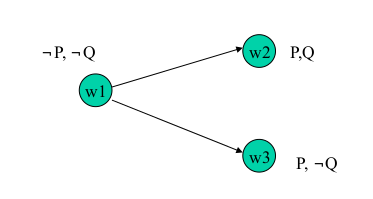
\includegraphics[width=.3\textwidth]{07/00}
\end{figure}

Certain types of agents decide what to do without reference to their history. They base their decision-making entirely on the present, with not reference at all to the past.\\
We will  call such agents \side{purely reactive} or \side{tropistic}, since they simply respond directly to their environment.

Given that tropistic agents makes decision based only on the present state of the environment, there is no reason for them to hold a state.

Formally, the behaviour of a purely reactive agent can be represented by a function
\[Ag: E\rightarrow Ac\]
A thermostat agent is an example of a purely reactive agent

\subsection{Agents with state}
A purely reactive agents is of no help to construct and implement agents, since its representation is extremely simple and abstract. For this reason, we need to refine our abstract model of agents, and make design choices that mostly relate to the sybsystems that go to make up an agent (i.e. what data and control structures will be present).

An \side{agent architecture} is eesentially a map of internals of an agent, its data structures, the operations that may be performed on these data structures and the control flow of between these data structures.\\
We are not partiularly interested in the content of an agent's state, but rather on the overall role of state in the agent's decision making loop.

\begin{figure}[!h]
\centering
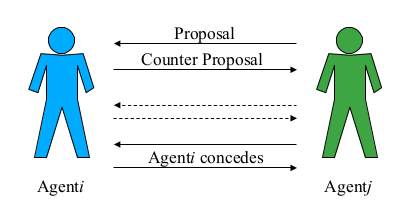
\includegraphics[width=.3\textwidth]{07/01}
\end{figure}

Thus agents have some internal data structure, which is tipically used to record information about the environment state and history. Let $I$ be the set of all internal state of the agent. An agent's decision-making process is then based, at least in part, on this information.

The perception function $see$ represents the agent's ability to obtain information from its environment. The output of the $see$ function is a $percept$ (perceptual input).\\
Let $Per$ be a non-empty set of percepts. Then $see$ is a functionof the form:
\[see: E\rightarrow Per\]
The action-selection function $action$ is defined as a mapping:
\[action : I \rightarrow Ac\]
from internal states to actions. An additional function $next$ is introduced, which maps an internal state and percept to an internal state:
\[next: I \times Per \rightarrow I\]
The behaviour of a state-based agent can be summarized in the following way:
\begin{enumerate}
\item The agent start in some initial internal state $i_0$
\item It observes its environment state $e$ and generates a percept $see(e)$
\item The internal state of the agent is then updated via the $next$ function
\[next(i_0, see(e))\]
\item The action selected by the agent is then 
\[action(next(i_0. see(e)))\]
\item This action is then performed, and the agent enters another cycle
\end{enumerate}

It is worth observing that state-based agents as defined here are in fact no more powerful than the standard agents we introduced earlier. In fact they are identical in their expressive power: every state-based agent can be transformed into a standard agent that is behaviourally equivalent.


\begin{figure}[!h]
\centering
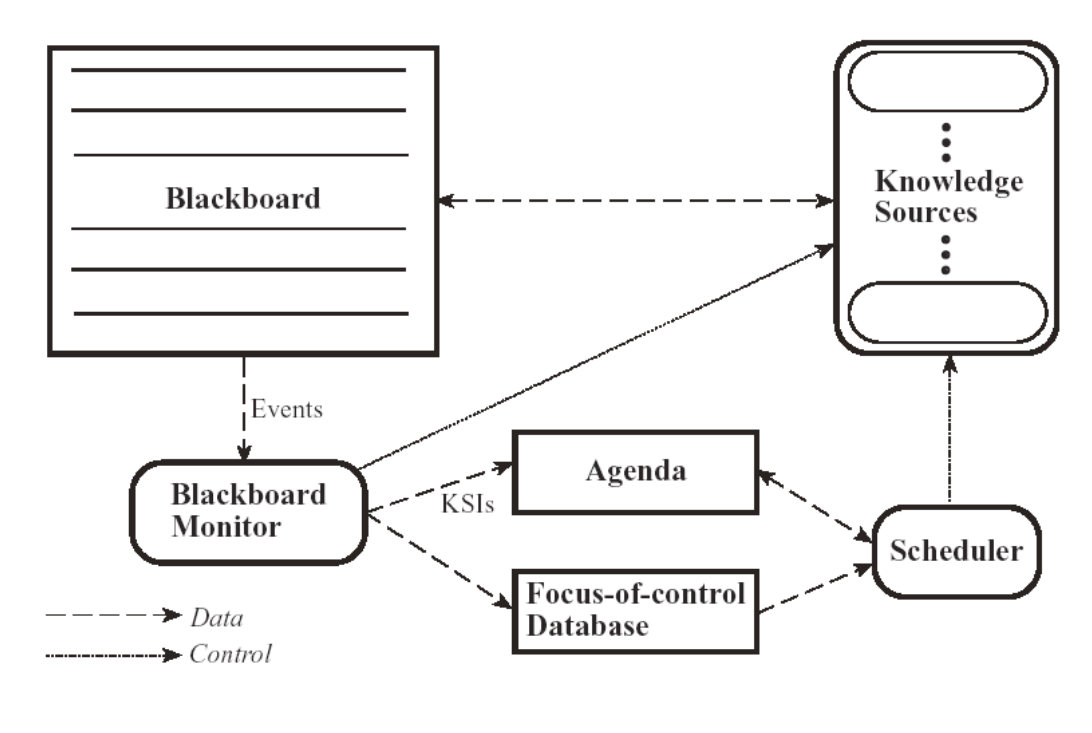
\includegraphics[width=.3\textwidth]{07/02}
\end{figure}

\section{Deliberative Architectures}
\subsection{Practical Reasoning}
The particular model of decision-making is known as \side{practical reasoning}. Practical reasoning is reasoning directed towards actions, or, in other terms, the process of figuring out what to do.

\say{Practical reasoning is a mattter of weighting conflicting considerations for and against competing options, where the relevant considerations are provided by what the agent desires/values/cares about and what the agent believes}.

It is important to distinguish practical reasoning from \side{theoretical reasoning}. Theoretical reasoning is directed towards beliefs. 

Human practical reasoning appears to consist of at least two distinct activities:
\begin{enumerate}
\item \side{Deliberation}: deciding what state of affairs we want to achieve
\item \side{Means-ends reasoning}: deciding how we want to achieve these states of affairs
\end{enumerate}

Hence, the output of the deliberation process are intentions, whereas the end result of means ends reasoning is a \side{plan} or \side{recipes} os some kind for achieving the chosen state of affairs.
\subsubsection{Deliberation}

First notice that it is possible to distinguish several different types of intention: actions and states of mind.

In this section, we will characterize intentions as states of mind or \side{future-directed intentions}, i.e. intentions that an agent has towards some future state of affairs.

The most obvious role of intentions is that they are pro-attitudes which means that they tend to lead to action.

The second main property of intentions is that they persist, i.e. If an agent adopt an intention, then the agent should persist with this intention and attempt to achieve it.

The third main property of intentions is that once an agent has adopted an intention, the very fact of having this intention will contrain its future practical reasoning. This means that an agent while holding a particular intention will not entertain options that are inconsisten with that intention.\\
This is a highly desirable property from the point of view of implementing rational agents, because in providing a \side{filter of admissibility}, intentions can be seen to constrain the space of possible intentions that an agent needs to consider.

Finally, intentions are closely related to beliefs about the future.

Form this discussion, we can identify the following closely related situations:
\begin{itemize}
\item Having an intention to bring about $\phi$, while believing that you will not bring about $\phi$, is called \side{intention-belief inconsistency}, and is not rational
\item Having an intention to achieve $\phi$ without believing that $\phi$ will be the case is \side{intention-belief incompleteness}, and is an acceptable property of rational agents
\end{itemize}

The distinction between these two cases is known as \side{asymmetry thesis}.\\
Summarizing, we can see that intentions play the following important roles in practical reasoning
\begin{itemize}
\item Intentions drive means-ends reasoning
\item Intentions persists
\item Intentions constrain future deliberation
\item Intentions influence belief upon which future practical reasoning is based
\end{itemize}

The process of deliberation or generation of intentions can be modelled via two functions:
\begin{itemize}
\item an \side{option generation} function\\
This function takes the agent's current beliefs and current intentions and on the basis of these produces a set of possible options and desires.
\item a \side{filtering} function\\
In order to select between competing options, an agent uses a filter function. Intuitively, the filter funciton must simplty select the best options for the agent to commit to.
\end{itemize}
Addiionally an agent's belief update process is modelled though a \side{belief revision function}

\subsubsection{Means-Ends Reasoning}
Means-ends reasoning is the process of deciding how to achieve an end/intention using the available means/actions.\\
Means ends reasoning is perhaps better known in the AI community as \side{planning}: planning is essentially automatic planning, in which a planner is a system that takes as input representations of the following:
\begin{itemize}
\item A goal, intention or a task
\item The current state of the environment: the agent's beliefs
\item The actions available to the agent
\end{itemize}
As output, a planning algorithm generates a plan.

The first real planner was the STRIPS system. The two basic components of STRIPS were :
\begin{enumerate}
\item a model of the world as a set of formulae of first-order logic 
\item a set of action chemata, which describe the preconditions and effects of all the actions available to the agent.
\end{enumerate}
The STRIPS planning algorithm was based on a principle of finding the difference between the current state of the world and the goal state, and reducing the difference by applying an action. Unfortunately, this proved to be an inefficient process for formulating plans, as STRIPS tended to become lost in low-level plan detail.
\subsubsection{Deductive Reasoning Agents}
The traditional approach to building artificially intelligent systems, known as symbolic AI, suggests that intelligent behaviour can be generated in a system by giving the system a symbolic representtion of its environmenta and its desired behaviour, and syntactically manipulating this representation.

Hence we define a \side{deliberative agent} or \side{deliberative agent architecture} to be one that:
\begin{itemize}
\item Contains an explicitly represented, symbolic model of the world
\item Makes decision via symbolic reasoning
\end{itemize}

In order to build such an agent, it seems we must solve two key problems:
\begin{itemize}
\item The \side{transduction problem}\\
The problem of translating the real world into an accurate, adequate symbolic description of the world, in time for that description to be useful
\item The \side{representation/ reasoning problem}\\
The problem of representing information symbolically, and getting agents to manipulate/reason with it, in time for the results to be useful.
\end{itemize}
\subsection{BDI - Belief, Desire, Intentions}
\begin{figure}[!h]
\centering
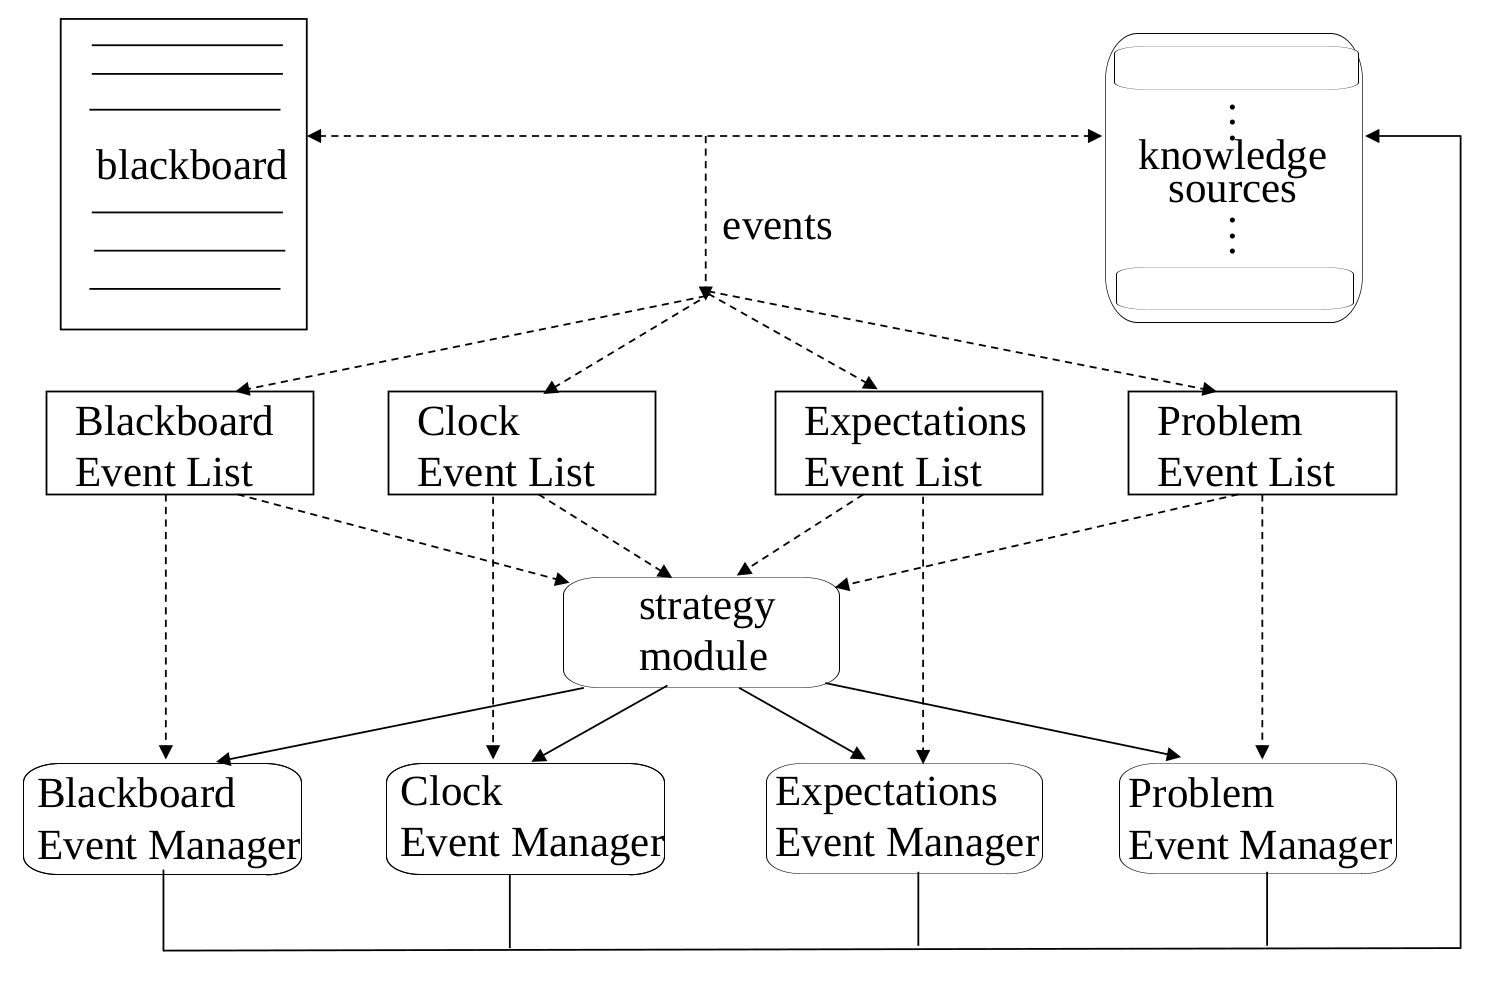
\includegraphics[width=.2\textwidth]{07/03}
\end{figure}
We can now discuss the overall control structuire of a practical reasoning agent. The basic strucutre of the decision-making process is a loop in which the agent continually:
\begin{itemize}
\item Observes the world and updates beliefs
\item deliberates to decide what intention to achieve
\item uses means-ends reasoning to find a plan to achieve these intentions
\item executes the plan
\end{itemize}

However, this basic control loop is complicated by a number of concerns. The first of these is that of commitment and, in particular, how committed an agent si to both ends (intentions) and means (the plan to achieve the intention)
\begin{lstlisting}[language=C++]
function action(p : E) : A
begin
	B := brf(B,p)
	D := options(B, I)
	I := filter(B,D,I)
	return execute(I)
end function action
\end{lstlisting}

\subsection{PRS - Procedural Reasoning Systems}
The \side{Procedural Reasoning System (PRS)} was perhaps the first agent architecture to explicitly embody the BDI paradigm, and proved to be the most durable agent architecture developed to date.

\begin{figure}[!h]
\centering
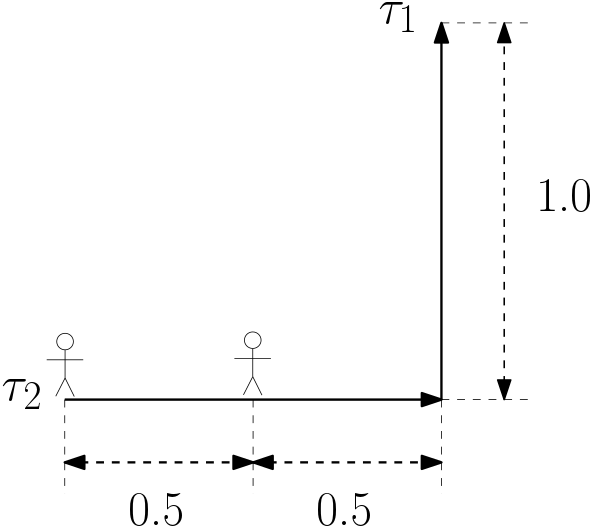
\includegraphics[width=.5\textwidth]{07/04}
\end{figure}

In the PRS, an agent does no planning from first principles. Instead, it is equipped with a library of pre-compiled plans (which effectively represent the agent's procedural knowledge). These plans are manually constructed, in advance, by the agent programmer.

Plans in the PRS each have the following components:
\begin{itemize}
\item A goal: the postcondition of the plan
\item A context: the precondition of the plan
\item A body: the recipe part of the plan or the course of action to carry out.
\end{itemize}
\subsection{IRMA - Intelligent Resource-Bounded Machine Architecture}
\begin{figure}[!h]
\centering
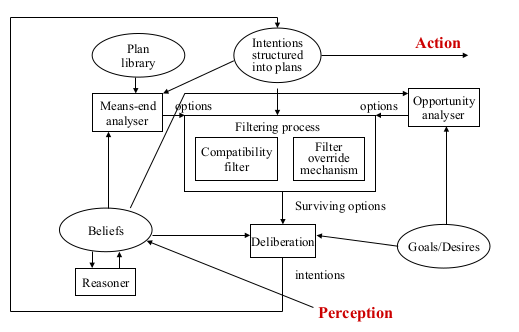
\includegraphics[width=.6\textwidth]{07/05}
\end{figure}
IRMA has 4 key symbolic data structures:
\begin{enumerate}
\item A plan library
\item Beliefs: information available to the agent
\item Goals/Desires: those things that the agent would like to make true
\item Intentions: goals/desires that the agent has chosen and committed to.
\end{enumerate}

Additionally, the architecture has:
\begin{itemize}
\item A reasoner: for reasoning about the world, an inference engine
\item A means-end analyser: determines which plans might be used to achieve the intentions
\item An opportunity analyser: monitors the environemnt and as a result of changes, generates new options
\item A filtering process: determines which options are compatible with current intentions
\item A deliberation process: responsible for deciding upon the best intentions to adopt
\end{itemize}


\section{Reactive Architectures}
The many problems with symbolic/logical approaches to building agent led some researchers to question and unltimately reject, the assumptions upon which such approaches are based.\\
In the mid to late 1980s, these researchers began to investigate alternatives to the symbolic AI paradigm. It is difficult to neatly characterize these different approaches, since their advocates are united mainly by a rejection of symbolic AI, rather than by a common manifesto. However, certain themes do recur:
\begin{itemize}
\item The rejection of symbolic representations and fo decision making based on syntactiv manipulation of such representations
\item The idea that intelligent, rational behaviour is seen as innately linked to the environment an agent occupies: intelligent behaviour is not disembodies but is a product of the interaction the agent maintains with its environment
\item The idea that intelligent behaviour emerges from the interaction of various simpler behaviours
\end{itemize}
Alternative appraches to agency are sometimes referred to as \side{behavioural situated} and \side{reactive} (because such systems are often perceived as simply reactive to an environment, without reasoning about it).

\subsection{The subsumption architecture	}
\phantom{c}\side{Subsumption architecture} is arguably the best-known reactive agent architecture.\\
It was developed by Rodney Brooks, who ahs propounded three key theses that have guided his work:
\begin{enumerate}
\item Intelligent behaviour can be generated without explicit representation of the kind that symbolic AI proposes
\item Intelligent behaviour can be generated wihout explicit abstract reasoning of the kind that symbolic AI proposes
\item Intelligence is an emergent property of certain complex systems
\end{enumerate}

Brooks also identifies two key ideas that have informed his research.
\begin{itemize}
\item \side{Situatedness and embodiment}: real intelligence is situated in the world, not in disembodies sytems such as theorem provers or expert systems
\item \side{Intelligence and emergence}: intelligent behaviour arises as a result of an agent's interaction with its environment. Also, intelligence is in the eye of the beholder, it is not an innate isolated property.
\end{itemize}

These ideas were made concrete in the subsumption architecture. There are two defining characteristics of the subsumption architecture. The first is that an agent's decision making is realized througha  set of task-accomplishing behaviours; each behaviour may be thought as an individual action seleciton function which continually takes perceptual input and maps it to an action to perform.\\
An important point to note is that these task-accomplishing modules are assumed to include no complex symbolic representation and are assumed to do no symbolic reasoning at all. In many implementations, these behaviours are implemented as rules which simply map perceptual input directly to actions. In this sense, the architecture is \textbf{reactive} and \textbf{situated} (since agents do not take past events into account and cannot forsee the future).

The second defining characteristic of the subsumption architecture is that many behaviours can fire simulataneously. There must obviously be a mechanism to choose between the different actions selected by these multiple actions.

Brooks propsoed arranging the modules into a \side{subsumption hierarchy}, with the behaviours arranged into \side{layers}. Lower players in thew hierarchy are able to inhibit higher layers (the lower the layer the higher the priority)
\subsubsection{Steel's Mars explorer experiments}

To illustrate the subsumption architecture in more detail, we will look at the Steels's Mars explorer experiments:
\say{The objective is to explore a distant planet – more concretely, to collect samples of a particular
type of precious rock. The location of the rock samples is not known in advance, but they are
typically clustered in certain spots. A number of autonomous vehicles are available that can
drive around the planet collecting samples and later re-enter a mother ship spacecraft to go back
to Earth. There is no detailed map of the planet available, although it is known that the terrain is
full of obstacles – hills, valleys, etc. – which prevent the vehicles from exchanging any
communication}

Steels's showed that the subsumption architecture would be a near optimal architecture for the individual agents.\\
The solution makes use of two mechanisms:
\begin{itemize}
\item The \side{gradient field}.\\
In order that agents can know in which direction the mother ship lies.
\item an \side{indirect communication method}
\end{itemize}
The behaviour of an individual agent is then built up from a number of behaviours. \\
For individual (non-cooperative) agents, the lowest-level behaviour is obstacle avoidance. The behaivour can be represented in the rule:
\begin{itemize}
\item Avoid obstacles
\item Any samples carried by agents are dropped back at the mother-ship
\item Agents carrying samples will return to the mother-ship
\item Agents will collecty samples they find
\item An agent with nothing better to do will explore randomly
\end{itemize}

\begin{lstlisting}[language=C++, mathescape=true]
function action(p : P) : A
begin
	fired := {$(c_i, a) | (c_i, a)\in R$ and $p \in c_i$}
	for each $(c_i,a) \in$ fired do
		if $\neg(\exists(c_{i-1}, a')\in$ fired such that $(c_{i-1}, a') < (c_i,a)$) then 
			return a
		end if
	end for
	return null
end function action
\end{lstlisting}

Where :
\begin{itemize}
\item $(c,a)$ is the condition action pair
\item R is the set of condition-action pairs
\item $c_1<c_2$ is read as $c_1$ is lower in hierarchy than  $c_2$
\end{itemize}

\subsection{Situated automata}
Rosenchein and Kaelbling pointed out that, just because we might conceptualize, of specify the behaviour of an agent in terms of concepts like beliefs and goals and indeed might use a logical representation of beliefs and goals to specify the agent, this does not implyt hat an agent must be implemented as a theorem prover for a logic of beliefs and goals.

In their \side{situated automata} paradigm, an agent is specified in a logic of beliefs and goals, but this specification is then compiled down to a digital machine, which satisfies the beliefs, goal specification in a precise formal sense.

The resulting digital machine can operate in a provably time-bounded fashion; it does not do any symbol manipulation, and in fact no symbol expressions are represented in the machine at all.\\
The logic used to specify an agent is essentially a logic of knowledge.

An agent is specified in terms of two components: perception and action.

Perception is specified by three components:
\begin{enumerate}
\item semantics of agent's input
\item a set of static facts
\item a specification of state transitions
\end{enumerate}
whereas action is specified by semantics of output.

The compiler syntheses a circuit whose output will have the correct semantics but that does not represent or manipulate symbolic expressions. This means that all symbolic manipulation is done at compile time.

\section{Hybrid Architectures}
Given the requirement that an agent be capable of reactive and proactive behaviour, an obvious decomposition involves creating separate subsystems to deal with these different types of behaivours.\\
This idea leads naturally to a class of architectures in which the various subsystems are arranged into a hierarchy of interacting layers.

Tipically, there will be at least two layers: to deal with reactive and proactive behaviours respectively. In principle, there is no reason why there should not be many more layers.\\
It is useful to characterize such architectures in terms of the information and control flows withing the layers. Broadly speaking, we can identify two types of control flow within layered architectures as follows:
\begin{itemize}
\item \side{Horizontal Layering}\\
In horizontally layered architectures, the software layers are each directly connected to the sensory input and action output. In effect each layer itself acts like an agent producing suggestions as to what action to perform
\item \side{Vertical Layering}\\
In vertically layered architectures, sensory input and action output are each dealt with by at most one layer
\end{itemize}

The great advantage of horizontally layered architectures is their conceptual simplicity: if we need an agent to exhibit n different types of behaivour then we implement n different layers. However, because the layers are each in effect competing with one another to generate action suggestions, there is a danger that the overall behaviour of the agent will not be coherent. In order to ensure conistency a \side{mediator} function, must decide about which layer has control of the agent at any given time.

Such central control is clearly difficult form a design point of view in any but the most simple system. The introduction of a central control system also introduces a bottleneck into the agents' decision making.

These problems are partly allievated in a vartically layeres achitecture. We can subdivide vertically layered architectures into:
\begin{itemize}
\item \side{one-pass architectures}\\
Control flows sequenctially through each layer, until the final layer generates action output
\item \side{two-pass architectures}\\
Information flows up the architecture (the first pass) and control then flows back down.
\end{itemize}
In both these architectures the complexity of interactions between layers is reduced and as a consequence it is much simpler than the horizontally layered case. However, this simplicity comes at the cost of some flexibility: in order for a vertically layered architecture to make a decision, control must pass between each different layer. This is not fault tolerant, i.e. failures in any one layer are likely to have serious consequences for agent performance.

\subsection{Touring Machines}
The \side{Touring Marchine architecture}, consists of three \side{actively producing layers}, i.e. each layer continually produces suggestions for what actions the agent should perform:
\begin{itemize}
\item the \side{reactive layer} provides a more-or-less immediate response to changes that occur in the environment. It is implemented as a set of situation-action rules similarly to the subsumption architecture.\\
These rules map sensor input directly to effector output. The rules can only make references to the agent's current state, but they cannot do any explicit reasoning about the world.

It is worth pointing out that the result of rules are actions not predicates, which means that if the rule fired, it would not result in any central environment model being update, but would just result in an action being suggested by the reactive layer.
\item the \side{planning layer} achieves the agent's proactive behaviour. Specifically, the planning layer is responsible for the running of the agent under normal circumstances.\\
The planning layer employs a library of plan `skeletons' called \side{schemas}, which are in essence hierarchically strcutured plans that the touring machines plannign layer elaborates at run-time in order to decide what to do.

So, in order to achieve a goal, the planning layer attempts to find a schema in its library which matches that goal. The schema will contain subgoals, which the planning layer elaborates by attempting to find other schemas in its plan library that match these subgoals
\item the \side{modelling layer} represents the various entities in the world (including the agent itself, as well as other agents). The modelling layer thus predicts conflicts between agents and generates new goals to be achieved in order to resolve these conflicts. Such goals are then passed to the planning layer.
\end{itemize}

\begin{figure}[!h]
\centering
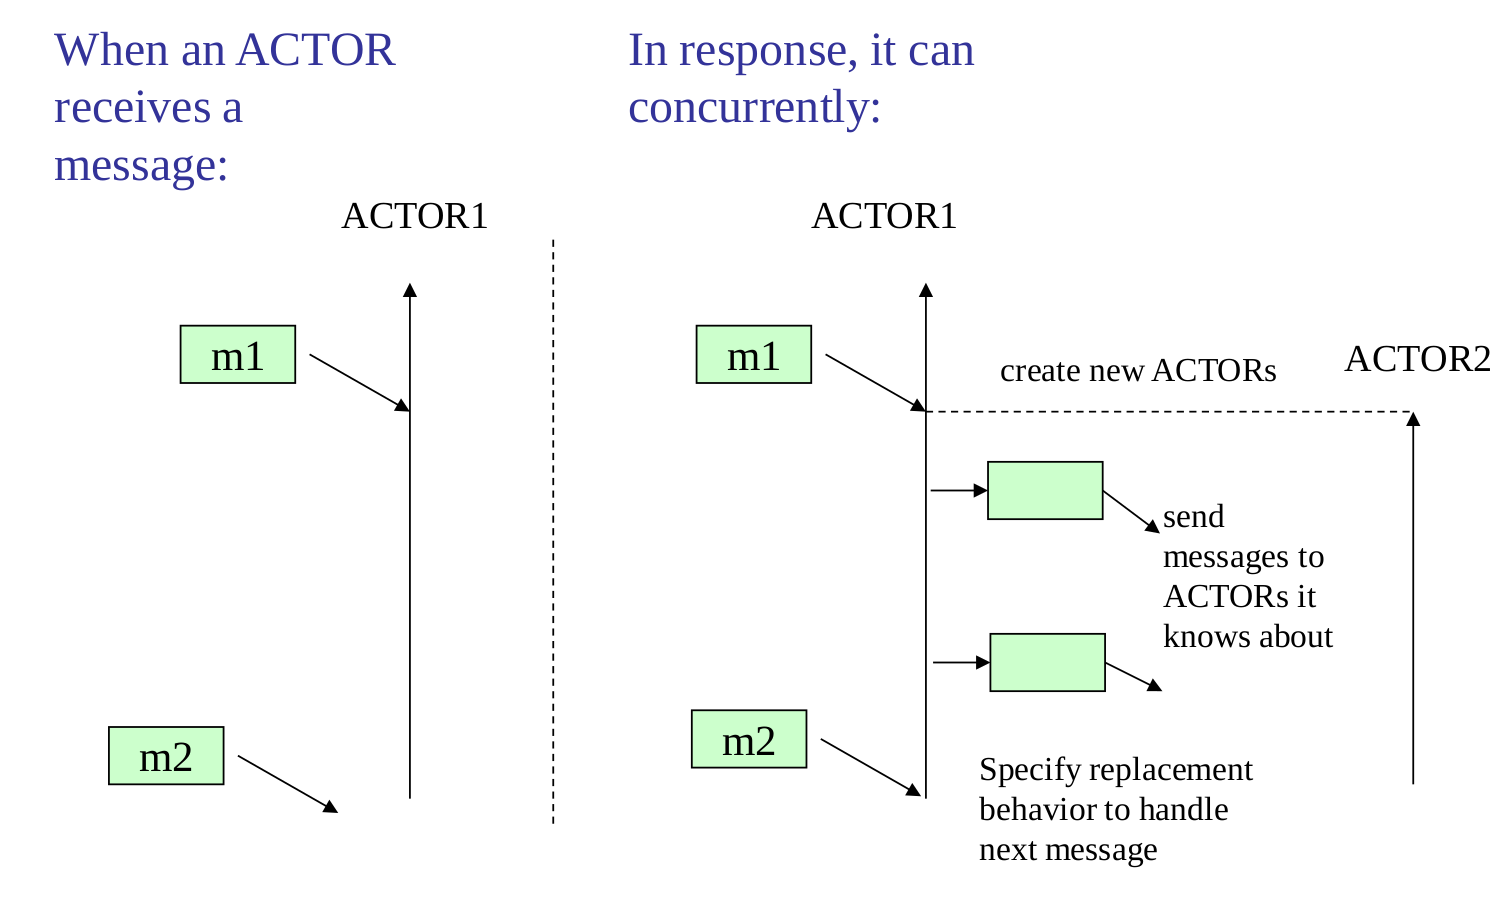
\includegraphics[width=.5\textwidth]{07/06}
\end{figure}

The three control layers are embedded within a control subsystem which is effectively responsible for deciding which of the layers should have control over the agent. This control subsystem is implemented as a set of control rules.\\
Control rules can either suppress sensor information between the control rules and the control layers, or else censor action outputs from the control layers.

\subsection{InteRRaP}
InteRRaP is a vertically layered two pass agent architecture that contrains three control layers.
The purpose of each InteRRaP layer apperas to be rather similar to the purpose of each corresponding Touring Machines layer.

\begin{figure}[!h]
\centering
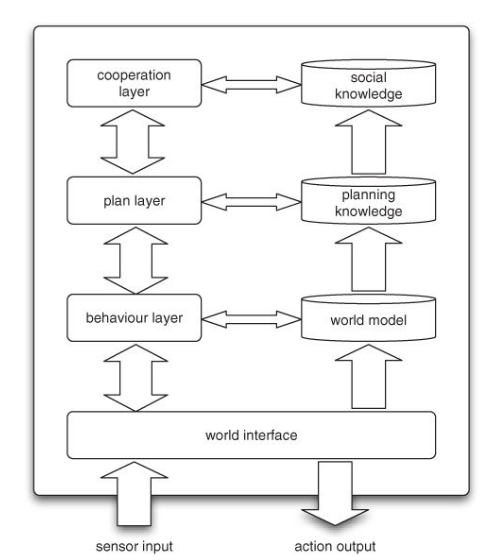
\includegraphics[width=.5\textwidth]{07/07}
\end{figure}

Thus :
\begin{itemize}
\item The lowest (\side{behaviour-based}) layer deals with reactive behaviour
\item The middle (\side{local planning}) layer deals with every day planning to achieve the agent's goals
\item The uppermost (\side{cooperative planning}) layer deals with social interactions.
\end{itemize}
Each layer has associated with it a knowledge base, i.e. a representation of the world appropriate for that layer. The se different knowledge bases represents the agent and its environment at different levels of abstraction.

Thus:
\begin{itemize}
\item The highest-level knowledge base represents the plans and actions of other agents in the environment
\item The middle-level knowledge base represents the plans and actions of the agent itself
\item The lowest-level knowledge base represents raw information about the environment
\end{itemize}
Layers interact with each other to achieve the same end. The two main types of interaction between layers are \side{bottom-up activation} and \side{top-down execution}. The former occurs when a lower layer passes control to a higher layer because it is not competent to deal with the current situation, the latter occurs when a higher layer makes use of the facilities provided by a lower layer to achieve one of its goals.

The basic flow of control in InteRRaP begins when perceptual input arrives at the lowest layer in the architecture.\\
If the reactive layer can deal with this input, then it will do so, otherwise, bottom-up activation will occur, and control will be passed to the local planning layer.\\
If the local planning layer can handle the situation, then it will do so, tipically by making use of top-down execution, otherwise, it will use bottom-up activation to pass control to the highest layer.

In this way, control in InteRRaP will flow from the lowest layer to higher layers of the architecture, and then back down again.

It is worth noting that each layer implements two general functions:
\begin{enumerate}
\item \side{situation recognition and goal activation} function which maps a knowledge base and current goals to a new set of goals
\item \side{planning and scheduling} function whcih is responsible for selecting which plans to execute, based on the current plans, goals, and knowledge base of that layer.
\end{enumerate}


